\documentclass[1p]{elsarticle_modified}
%\bibliographystyle{elsarticle-num}

%\usepackage[colorlinks]{hyperref}
%\usepackage{abbrmath_seonhwa} %\Abb, \Ascr, \Acal ,\Abf, \Afrak
\usepackage{amsfonts}
\usepackage{amssymb}
\usepackage{amsmath}
\usepackage{amsthm}
\usepackage{scalefnt}
\usepackage{amsbsy}
\usepackage{kotex}
\usepackage{caption}
\usepackage{subfig}
\usepackage{color}
\usepackage{graphicx}
\usepackage{xcolor} %% white, black, red, green, blue, cyan, magenta, yellow
\usepackage{float}
\usepackage{setspace}
\usepackage{hyperref}

\usepackage{tikz}
\usetikzlibrary{arrows}

\usepackage{multirow}
\usepackage{array} % fixed length table
\usepackage{hhline}

%%%%%%%%%%%%%%%%%%%%%
\makeatletter
\renewcommand*\env@matrix[1][\arraystretch]{%
	\edef\arraystretch{#1}%
	\hskip -\arraycolsep
	\let\@ifnextchar\new@ifnextchar
	\array{*\c@MaxMatrixCols c}}
\makeatother %https://tex.stackexchange.com/questions/14071/how-can-i-increase-the-line-spacing-in-a-matrix
%%%%%%%%%%%%%%%

\usepackage[normalem]{ulem}

\newcommand{\msout}[1]{\ifmmode\text{\sout{\ensuremath{#1}}}\else\sout{#1}\fi}
%SOURCE: \msout is \stkout macro in https://tex.stackexchange.com/questions/20609/strikeout-in-math-mode

\newcommand{\cancel}[1]{
	\ifmmode
	{\color{red}\msout{#1}}
	\else
	{\color{red}\sout{#1}}
	\fi
}

\newcommand{\add}[1]{
	{\color{blue}\uwave{#1}}
}

\newcommand{\replace}[2]{
	\ifmmode
	{\color{red}\msout{#1}}{\color{blue}\uwave{#2}}
	\else
	{\color{red}\sout{#1}}{\color{blue}\uwave{#2}}
	\fi
}

\newcommand{\Sol}{\mathcal{S}} %segment
\newcommand{\D}{D} %diagram
\newcommand{\A}{\mathcal{A}} %arc


%%%%%%%%%%%%%%%%%%%%%%%%%%%%%5 test

\def\sl{\operatorname{\textup{SL}}(2,\Cbb)}
\def\psl{\operatorname{\textup{PSL}}(2,\Cbb)}
\def\quan{\mkern 1mu \triangleright \mkern 1mu}

\theoremstyle{definition}
\newtheorem{thm}{Theorem}[section]
\newtheorem{prop}[thm]{Proposition}
\newtheorem{lem}[thm]{Lemma}
\newtheorem{ques}[thm]{Question}
\newtheorem{cor}[thm]{Corollary}
\newtheorem{defn}[thm]{Definition}
\newtheorem{exam}[thm]{Example}
\newtheorem{rmk}[thm]{Remark}
\newtheorem{alg}[thm]{Algorithm}

\newcommand{\I}{\sqrt{-1}}
\begin{document}

%\begin{frontmatter}
%
%\title{Boundary parabolic representations of knots up to 8 crossings}
%
%%% Group authors per affiliation:
%\author{Yunhi Cho} 
%\address{Department of Mathematics, University of Seoul, Seoul, Korea}
%\ead{yhcho@uos.ac.kr}
%
%
%\author{Seonhwa Kim} %\fnref{s_kim}}
%\address{Center for Geometry and Physics, Institute for Basic Science, Pohang, 37673, Korea}
%\ead{ryeona17@ibs.re.kr}
%
%\author{Hyuk Kim}
%\address{Department of Mathematical Sciences, Seoul National University, Seoul 08826, Korea}
%\ead{hyukkim@snu.ac.kr}
%
%\author{Seokbeom Yoon}
%\address{Department of Mathematical Sciences, Seoul National University, Seoul, 08826,  Korea}
%\ead{sbyoon15@snu.ac.kr}
%
%\begin{abstract}
%We find all boundary parabolic representation of knots up to 8 crossings.
%
%\end{abstract}
%\begin{keyword}
%    \MSC[2010] 57M25 
%\end{keyword}
%
%\end{frontmatter}

%\linenumbers
%\tableofcontents
%
\newcommand\colored[1]{\textcolor{white}{\rule[-0.35ex]{0.8em}{1.4ex}}\kern-0.8em\color{red} #1}%
%\newcommand\colored[1]{\textcolor{white}{ #1}\kern-2.17ex	\textcolor{white}{ #1}\kern-1.81ex	\textcolor{white}{ #1}\kern-2.15ex\color{red}#1	}

{\Large $\underline{12a_{0869}~(K12a_{0869})}$}

\setlength{\tabcolsep}{10pt}
\renewcommand{\arraystretch}{1.6}
\vspace{1cm}\begin{tabular}{m{100pt}>{\centering\arraybackslash}m{274pt}}
\multirow{5}{120pt}{
	\centering
	\includegraphics[width=112pt]{../../../GIT/diagram.site/Diagrams/png/1670_12a_0869.png}\\
\ \ \ A knot diagram\footnotemark}&
\allowdisplaybreaks
\textbf{Linearized knot diagam} \\
\cline{2-2}
 &
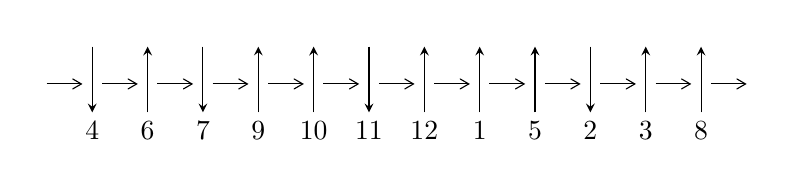
\begin{tikzpicture}[x=20pt, y=17pt]
	% nodes
	\node (C0) at (0, 0) {};
	\node (C1) at (1, 0) {};
	\node (C1U) at (1, +1) {};
	\node (C1D) at (1, -1) {4};

	\node (C2) at (2, 0) {};
	\node (C2U) at (2, +1) {};
	\node (C2D) at (2, -1) {6};

	\node (C3) at (3, 0) {};
	\node (C3U) at (3, +1) {};
	\node (C3D) at (3, -1) {7};

	\node (C4) at (4, 0) {};
	\node (C4U) at (4, +1) {};
	\node (C4D) at (4, -1) {9};

	\node (C5) at (5, 0) {};
	\node (C5U) at (5, +1) {};
	\node (C5D) at (5, -1) {10};

	\node (C6) at (6, 0) {};
	\node (C6U) at (6, +1) {};
	\node (C6D) at (6, -1) {11};

	\node (C7) at (7, 0) {};
	\node (C7U) at (7, +1) {};
	\node (C7D) at (7, -1) {12};

	\node (C8) at (8, 0) {};
	\node (C8U) at (8, +1) {};
	\node (C8D) at (8, -1) {1};

	\node (C9) at (9, 0) {};
	\node (C9U) at (9, +1) {};
	\node (C9D) at (9, -1) {5};

	\node (C10) at (10, 0) {};
	\node (C10U) at (10, +1) {};
	\node (C10D) at (10, -1) {2};

	\node (C11) at (11, 0) {};
	\node (C11U) at (11, +1) {};
	\node (C11D) at (11, -1) {3};

	\node (C12) at (12, 0) {};
	\node (C12U) at (12, +1) {};
	\node (C12D) at (12, -1) {8};
	\node (C13) at (13, 0) {};

	% arrows
	\draw[->,>={angle 60}]
	(C0) edge (C1) (C1) edge (C2) (C2) edge (C3) (C3) edge (C4) (C4) edge (C5) (C5) edge (C6) (C6) edge (C7) (C7) edge (C8) (C8) edge (C9) (C9) edge (C10) (C10) edge (C11) (C11) edge (C12) (C12) edge (C13) ;	\draw[->,>=stealth]
	(C1U) edge (C1D) (C2D) edge (C2U) (C3U) edge (C3D) (C4D) edge (C4U) (C5D) edge (C5U) (C6U) edge (C6D) (C7D) edge (C7U) (C8D) edge (C8U) (C9D) edge (C9U) (C10U) edge (C10D) (C11D) edge (C11U) (C12D) edge (C12U) ;
	\end{tikzpicture} \\
\hhline{~~} \\& 
\textbf{Solving Sequence} \\ \cline{2-2} 
 &
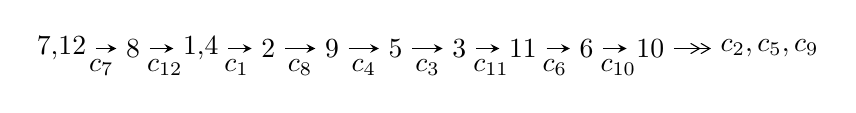
\begin{tikzpicture}[x=23pt, y=7pt]
	% node
	\node (A0) at (-1/8, 0) {7,12};
	\node (A1) at (1, 0) {8};
	\node (A2) at (33/16, 0) {1,4};
	\node (A3) at (25/8, 0) {2};
	\node (A4) at (33/8, 0) {9};
	\node (A5) at (41/8, 0) {5};
	\node (A6) at (49/8, 0) {3};
	\node (A7) at (57/8, 0) {11};
	\node (A8) at (65/8, 0) {6};
	\node (A9) at (73/8, 0) {10};
	\node (C1) at (1/2, -1) {$c_{7}$};
	\node (C2) at (3/2, -1) {$c_{12}$};
	\node (C3) at (21/8, -1) {$c_{1}$};
	\node (C4) at (29/8, -1) {$c_{8}$};
	\node (C5) at (37/8, -1) {$c_{4}$};
	\node (C6) at (45/8, -1) {$c_{3}$};
	\node (C7) at (53/8, -1) {$c_{11}$};
	\node (C8) at (61/8, -1) {$c_{6}$};
	\node (C9) at (69/8, -1) {$c_{10}$};
	\node (A10) at (11, 0) {$c_{2},c_{5},c_{9}$};

	% edge
	\draw[->,>=stealth]	
	(A0) edge (A1) (A1) edge (A2) (A2) edge (A3) (A3) edge (A4) (A4) edge (A5) (A5) edge (A6) (A6) edge (A7) (A7) edge (A8) (A8) edge (A9) ;
	\draw[->>,>={angle 60}]	
	(A9) edge (A10);
\end{tikzpicture} \\ 

\end{tabular} \\

\footnotetext{
The image of knot diagram is generated by the software ``\textbf{Draw programme}" developed by Andrew Bartholomew(\url{http://www.layer8.co.uk/maths/draw/index.htm\#Running-draw}), where we modified some parts for our purpose(\url{https://github.com/CATsTAILs/LinksPainter}).
}\phantom \\ \newline 
\centering \textbf{Ideals for irreducible components\footnotemark of $X_{\text{par}}$} 
 
\begin{align*}
I^u_{1}&=\langle 
-959 u^{21}+8 u^{20}+\cdots+6991 b-10004,\;12718 u^{21}+1556 u^{20}+\cdots+6991 a+39666,\\
\phantom{I^u_{1}}&\phantom{= \langle  }u^{22}-14 u^{20}+\cdots+2 u-1\rangle \\
I^u_{2}&=\langle 
-1.39235\times10^{140} u^{77}+6.32801\times10^{139} u^{76}+\cdots+1.95985\times10^{140} b-2.88234\times10^{142},\\
\phantom{I^u_{2}}&\phantom{= \langle  }6.63657\times10^{141} u^{77}-2.91804\times10^{141} u^{76}+\cdots+8.42734\times10^{141} a+1.55560\times10^{144},\\
\phantom{I^u_{2}}&\phantom{= \langle  }u^{78}-2 u^{77}+\cdots+136 u-43\rangle \\
I^u_{3}&=\langle 
- u^7+4 u^5-5 u^3- u^2+b+u+1,\;u^7- u^6-4 u^5+4 u^4+5 u^3-4 u^2+a- u,\\
\phantom{I^u_{3}}&\phantom{= \langle  }u^8-5 u^6+8 u^4+u^3-3 u^2-2 u-1\rangle \\
I^u_{4}&=\langle 
2 u^7-4 u^6-5 u^5+11 u^4- u^3-3 u^2+b+5 u-3,\;-3 u^7+6 u^6+8 u^5-18 u^4+u^3+8 u^2+a-8 u+4,\\
\phantom{I^u_{4}}&\phantom{= \langle  }u^8-3 u^7- u^6+9 u^5-5 u^4-3 u^3+4 u^2-4 u+1\rangle \\
I^u_{5}&=\langle 
- u^3+b+2 u-2,\;2 u^3+2 u^2+a-3 u-1,\;u^4+2 u^3- u^2-2 u+1\rangle \\
\\
\end{align*}
\raggedright * 5 irreducible components of $\dim_{\mathbb{C}}=0$, with total 120 representations.\\
\footnotetext{All coefficients of polynomials are rational numbers. But the coefficients are sometimes approximated in decimal forms when there is not enough margin.}
\newpage
\renewcommand{\arraystretch}{1}
\centering \section*{I. $I^u_{1}= \langle -959 u^{21}+8 u^{20}+\cdots+6991 b-10004,\;12718 u^{21}+1556 u^{20}+\cdots+6991 a+39666,\;u^{22}-14 u^{20}+\cdots+2 u-1 \rangle$}
\flushleft \textbf{(i) Arc colorings}\\
\begin{tabular}{m{7pt} m{180pt} m{7pt} m{180pt} }
\flushright $a_{7}=$&$\begin{pmatrix}1\\0\end{pmatrix}$ \\
\flushright $a_{12}=$&$\begin{pmatrix}0\\u\end{pmatrix}$ \\
\flushright $a_{8}=$&$\begin{pmatrix}1\\- u^2\end{pmatrix}$ \\
\flushright $a_{1}=$&$\begin{pmatrix}u\\- u^3+u\end{pmatrix}$ \\
\flushright $a_{4}=$&$\begin{pmatrix}-1.81920 u^{21}-0.222572 u^{20}+\cdots-0.747533 u-5.67387\\0.137176 u^{21}-0.00114433 u^{20}+\cdots+2.09898 u+1.43098\end{pmatrix}$ \\
\flushright $a_{2}=$&$\begin{pmatrix}-1.06737 u^{21}-1.55314 u^{20}+\cdots+1.34659 u-1.79874\\0.447575 u^{21}+0.521814 u^{20}+\cdots-0.136890 u+2.47189\end{pmatrix}$ \\
\flushright $a_{9}=$&$\begin{pmatrix}- u^2+1\\u^4-2 u^2\end{pmatrix}$ \\
\flushright $a_{5}=$&$\begin{pmatrix}-1.81920 u^{21}-0.222572 u^{20}+\cdots+0.252467 u-5.67387\\0.137176 u^{21}-0.00114433 u^{20}+\cdots+2.09898 u+1.43098\end{pmatrix}$ \\
\flushright $a_{3}=$&$\begin{pmatrix}-1.68202 u^{21}-0.223716 u^{20}+\cdots+1.35145 u-4.24288\\0.137176 u^{21}-0.00114433 u^{20}+\cdots+2.09898 u+1.43098\end{pmatrix}$ \\
\flushright $a_{11}=$&$\begin{pmatrix}1.25819 u^{21}+0.476470 u^{20}+\cdots-0.714633 u+2.67458\\0.733085 u^{21}-0.0321842 u^{20}+\cdots+1.28394 u+0.746388\end{pmatrix}$ \\
\flushright $a_{6}=$&$\begin{pmatrix}2.00458 u^{21}+1.20956 u^{20}+\cdots-2.62652 u+5.45129\\-0.439565 u^{21}-0.405092 u^{20}+\cdots-1.95952 u-1.43213\end{pmatrix}$ \\
\flushright $a_{10}=$&$\begin{pmatrix}0.222572 u^{21}-0.185381 u^{20}+\cdots+2.03547 u+2.81920\\0.00114433 u^{21}+0.302389 u^{20}+\cdots-1.15663 u-0.137176\end{pmatrix}$\\&\end{tabular}
\flushleft \textbf{(ii) Obstruction class $= -1$}\\~\\
\flushleft \textbf{(iii) Cusp Shapes $= -\frac{44709}{6991} u^{21}-\frac{15293}{6991} u^{20}+\cdots-\frac{71860}{6991} u-\frac{27948}{6991}$}\\~\\
\newpage\renewcommand{\arraystretch}{1}
\flushleft \textbf{(iv) u-Polynomials at the component}\newline \\
\begin{tabular}{m{50pt}|m{274pt}}
Crossings & \hspace{64pt}u-Polynomials at each crossing \\
\hline $$\begin{aligned}c_{1}\end{aligned}$$&$\begin{aligned}
&u^{22}-18 u^{21}+\cdots-1136 u+64
\end{aligned}$\\
\hline $$\begin{aligned}c_{2},c_{11}\end{aligned}$$&$\begin{aligned}
&u^{22}+u^{21}+\cdots-5 u+1
\end{aligned}$\\
\hline $$\begin{aligned}c_{3},c_{10}\end{aligned}$$&$\begin{aligned}
&u^{22}+u^{21}+\cdots-6 u^2+1
\end{aligned}$\\
\hline $$\begin{aligned}c_{4},c_{5},c_{7}\\c_{8},c_{9},c_{12}\end{aligned}$$&$\begin{aligned}
&u^{22}-14 u^{20}+\cdots-2 u-1
\end{aligned}$\\
\hline $$\begin{aligned}c_{6}\end{aligned}$$&$\begin{aligned}
&u^{22}-11 u^{21}+\cdots-60 u+8
\end{aligned}$\\
\hline
\end{tabular}\\~\\
\newpage\renewcommand{\arraystretch}{1}
\flushleft \textbf{(v) Riley Polynomials at the component}\newline \\
\begin{tabular}{m{50pt}|m{274pt}}
Crossings & \hspace{64pt}Riley Polynomials at each crossing \\
\hline $$\begin{aligned}c_{1}\end{aligned}$$&$\begin{aligned}
&y^{22}+94 y^{20}+\cdots-435456 y+4096
\end{aligned}$\\
\hline $$\begin{aligned}c_{2},c_{11}\end{aligned}$$&$\begin{aligned}
&y^{22}-17 y^{21}+\cdots-21 y+1
\end{aligned}$\\
\hline $$\begin{aligned}c_{3},c_{10}\end{aligned}$$&$\begin{aligned}
&y^{22}+3 y^{21}+\cdots-12 y+1
\end{aligned}$\\
\hline $$\begin{aligned}c_{4},c_{5},c_{7}\\c_{8},c_{9},c_{12}\end{aligned}$$&$\begin{aligned}
&y^{22}-28 y^{21}+\cdots-26 y+1
\end{aligned}$\\
\hline $$\begin{aligned}c_{6}\end{aligned}$$&$\begin{aligned}
&y^{22}-5 y^{21}+\cdots-1168 y+64
\end{aligned}$\\
\hline
\end{tabular}\\~\\
\newpage\flushleft \textbf{(vi) Complex Volumes and Cusp Shapes}
$$\begin{array}{c|c|c}  
\text{Solutions to }I^u_{1}& \I (\text{vol} + \sqrt{-1}CS) & \text{Cusp shape}\\
 \hline 
\begin{aligned}
u &= \phantom{-}0.620777 + 0.699897 I \\
a &= -0.444548 - 0.589843 I \\
b &= -0.975241 + 0.924812 I\end{aligned}
 & \phantom{-}0.28538 + 9.52077 I & \phantom{-}5.54038 - 10.18443 I \\ \hline\begin{aligned}
u &= \phantom{-}0.620777 - 0.699897 I \\
a &= -0.444548 + 0.589843 I \\
b &= -0.975241 - 0.924812 I\end{aligned}
 & \phantom{-}0.28538 - 9.52077 I & \phantom{-}5.54038 + 10.18443 I \\ \hline\begin{aligned}
u &= -0.543470 + 0.600696 I \\
a &= \phantom{-}0.287139 - 0.161144 I \\
b &= \phantom{-}0.162955 + 0.882903 I\end{aligned}
 & \phantom{-}2.06715 - 1.71752 I & \phantom{-}11.74245 + 5.24817 I \\ \hline\begin{aligned}
u &= -0.543470 - 0.600696 I \\
a &= \phantom{-}0.287139 + 0.161144 I \\
b &= \phantom{-}0.162955 - 0.882903 I\end{aligned}
 & \phantom{-}2.06715 + 1.71752 I & \phantom{-}11.74245 - 5.24817 I \\ \hline\begin{aligned}
u &= -0.616708 + 0.440990 I \\
a &= -1.099990 - 0.644526 I \\
b &= \phantom{-}0.481328 - 0.475392 I\end{aligned}
 & \phantom{-}0.165742 + 1.104130 I & \phantom{-}7.76898 - 0.48945 I \\ \hline\begin{aligned}
u &= -0.616708 - 0.440990 I \\
a &= -1.099990 + 0.644526 I \\
b &= \phantom{-}0.481328 + 0.475392 I\end{aligned}
 & \phantom{-}0.165742 - 1.104130 I & \phantom{-}7.76898 + 0.48945 I \\ \hline\begin{aligned}
u &= -0.688001\phantom{ +0.000000I} \\
a &= -0.0816056\phantom{ +0.000000I} \\
b &= -1.19439\phantom{ +0.000000I}\end{aligned}
 & \phantom{-}0.164932\phantom{ +0.000000I} & \phantom{-}13.5940\phantom{ +0.000000I} \\ \hline\begin{aligned}
u &= \phantom{-}1.47278 + 0.24907 I \\
a &= \phantom{-}0.639561 + 0.759382 I \\
b &= -0.461601 - 0.642988 I\end{aligned}
 & \phantom{-}8.63753 + 2.31951 I & \phantom{-}6.80409 + 2.73514 I \\ \hline\begin{aligned}
u &= \phantom{-}1.47278 - 0.24907 I \\
a &= \phantom{-}0.639561 - 0.759382 I \\
b &= -0.461601 + 0.642988 I\end{aligned}
 & \phantom{-}8.63753 - 2.31951 I & \phantom{-}6.80409 - 2.73514 I \\ \hline\begin{aligned}
u &= -0.479173\phantom{ +0.000000I} \\
a &= -0.636420\phantom{ +0.000000I} \\
b &= -0.286181\phantom{ +0.000000I}\end{aligned}
 & \phantom{-}0.816563\phantom{ +0.000000I} & \phantom{-}11.9280\phantom{ +0.000000I}\\
 \hline 
 \end{array}$$\newpage$$\begin{array}{c|c|c}  
\text{Solutions to }I^u_{1}& \I (\text{vol} + \sqrt{-1}CS) & \text{Cusp shape}\\
 \hline 
\begin{aligned}
u &= \phantom{-}1.52797 + 0.02574 I \\
a &= -0.26700 + 1.87402 I \\
b &= -0.755859 - 1.019260 I\end{aligned}
 & \phantom{-}14.2021 - 4.2069 I & \phantom{-}12.43580 + 5.16700 I \\ \hline\begin{aligned}
u &= \phantom{-}1.52797 - 0.02574 I \\
a &= -0.26700 - 1.87402 I \\
b &= -0.755859 + 1.019260 I\end{aligned}
 & \phantom{-}14.2021 + 4.2069 I & \phantom{-}12.43580 - 5.16700 I \\ \hline\begin{aligned}
u &= \phantom{-}0.357972 + 0.207376 I \\
a &= \phantom{-}2.77142 + 1.51494 I \\
b &= \phantom{-}0.416028 - 0.835216 I\end{aligned}
 & \phantom{-}1.27965 + 3.66433 I & \phantom{-}15.0331 - 10.2324 I \\ \hline\begin{aligned}
u &= \phantom{-}0.357972 - 0.207376 I \\
a &= \phantom{-}2.77142 - 1.51494 I \\
b &= \phantom{-}0.416028 + 0.835216 I\end{aligned}
 & \phantom{-}1.27965 - 3.66433 I & \phantom{-}15.0331 + 10.2324 I \\ \hline\begin{aligned}
u &= -1.59329 + 0.06074 I \\
a &= -0.215693 + 0.896227 I \\
b &= \phantom{-}0.973496 - 0.770109 I\end{aligned}
 & \phantom{-}15.7122 - 0.5131 I & \phantom{-}13.84357 - 0.14086 I \\ \hline\begin{aligned}
u &= -1.59329 - 0.06074 I \\
a &= -0.215693 - 0.896227 I \\
b &= \phantom{-}0.973496 + 0.770109 I\end{aligned}
 & \phantom{-}15.7122 + 0.5131 I & \phantom{-}13.84357 + 0.14086 I \\ \hline\begin{aligned}
u &= -1.60156\phantom{ +0.000000I} \\
a &= \phantom{-}0.521347\phantom{ +0.000000I} \\
b &= \phantom{-}0.540591\phantom{ +0.000000I}\end{aligned}
 & \phantom{-}15.7785\phantom{ +0.000000I} & \phantom{-}15.7070\phantom{ +0.000000I} \\ \hline\begin{aligned}
u &= \phantom{-}1.63321 + 0.25925 I \\
a &= -0.25245 + 1.62291 I \\
b &= \phantom{-}1.21002 - 1.23023 I\end{aligned}
 & \phantom{-}15.4855 + 16.9496 I & \phantom{-}10.93128 - 7.84709 I \\ \hline\begin{aligned}
u &= \phantom{-}1.63321 - 0.25925 I \\
a &= -0.25245 - 1.62291 I \\
b &= \phantom{-}1.21002 + 1.23023 I\end{aligned}
 & \phantom{-}15.4855 - 16.9496 I & \phantom{-}10.93128 + 7.84709 I \\ \hline\begin{aligned}
u &= -1.64240 + 0.25438 I \\
a &= -0.026921 + 1.355890 I \\
b &= -0.57852 - 1.30048 I\end{aligned}
 & \phantom{-}17.0516 - 8.7183 I & \phantom{-}13.8836 + 4.8126 I\\
 \hline 
 \end{array}$$\newpage$$\begin{array}{c|c|c}  
\text{Solutions to }I^u_{1}& \I (\text{vol} + \sqrt{-1}CS) & \text{Cusp shape}\\
 \hline 
\begin{aligned}
u &= -1.64240 - 0.25438 I \\
a &= -0.026921 - 1.355890 I \\
b &= -0.57852 + 1.30048 I\end{aligned}
 & \phantom{-}17.0516 + 8.7183 I & \phantom{-}13.8836 - 4.8126 I \\ \hline\begin{aligned}
u &= \phantom{-}0.335041\phantom{ +0.000000I} \\
a &= -2.58634\phantom{ +0.000000I} \\
b &= \phantom{-}0.994760\phantom{ +0.000000I}\end{aligned}
 & -2.04032\phantom{ +0.000000I} & -5.19480\phantom{ +0.000000I}\\
 \hline 
 \end{array}$$\newpage\newpage\renewcommand{\arraystretch}{1}
\centering \section*{II. $I^u_{2}= \langle -1.39\times10^{140} u^{77}+6.33\times10^{139} u^{76}+\cdots+1.96\times10^{140} b-2.88\times10^{142},\;6.64\times10^{141} u^{77}-2.92\times10^{141} u^{76}+\cdots+8.43\times10^{141} a+1.56\times10^{144},\;u^{78}-2 u^{77}+\cdots+136 u-43 \rangle$}
\flushleft \textbf{(i) Arc colorings}\\
\begin{tabular}{m{7pt} m{180pt} m{7pt} m{180pt} }
\flushright $a_{7}=$&$\begin{pmatrix}1\\0\end{pmatrix}$ \\
\flushright $a_{12}=$&$\begin{pmatrix}0\\u\end{pmatrix}$ \\
\flushright $a_{8}=$&$\begin{pmatrix}1\\- u^2\end{pmatrix}$ \\
\flushright $a_{1}=$&$\begin{pmatrix}u\\- u^3+u\end{pmatrix}$ \\
\flushright $a_{4}=$&$\begin{pmatrix}-0.787505 u^{77}+0.346259 u^{76}+\cdots+138.255 u-184.590\\0.710437 u^{77}-0.322883 u^{76}+\cdots-127.381 u+147.069\end{pmatrix}$ \\
\flushright $a_{2}=$&$\begin{pmatrix}-2.36422 u^{77}+3.85705 u^{76}+\cdots+112.872 u-279.876\\-0.790784 u^{77}+0.595382 u^{76}+\cdots+100.423 u-123.684\end{pmatrix}$ \\
\flushright $a_{9}=$&$\begin{pmatrix}- u^2+1\\u^4-2 u^2\end{pmatrix}$ \\
\flushright $a_{5}=$&$\begin{pmatrix}-0.510367 u^{77}+0.427296 u^{76}+\cdots+63.1806 u-113.051\\0.677512 u^{77}-0.534118 u^{76}+\cdots-97.2276 u+120.573\end{pmatrix}$ \\
\flushright $a_{3}=$&$\begin{pmatrix}-0.0770682 u^{77}+0.0233760 u^{76}+\cdots+10.8743 u-37.5207\\0.710437 u^{77}-0.322883 u^{76}+\cdots-127.381 u+147.069\end{pmatrix}$ \\
\flushright $a_{11}=$&$\begin{pmatrix}-1.01566 u^{77}+2.13882 u^{76}+\cdots-56.8939 u-95.6811\\1.96720 u^{77}-4.01917 u^{76}+\cdots-55.8889 u+149.806\end{pmatrix}$ \\
\flushright $a_{6}=$&$\begin{pmatrix}4.21314 u^{77}-6.18031 u^{76}+\cdots-353.473 u+453.881\\1.88902 u^{77}-0.366972 u^{76}+\cdots-387.504 u+407.067\end{pmatrix}$ \\
\flushright $a_{10}=$&$\begin{pmatrix}0.555335 u^{77}-0.588323 u^{76}+\cdots-78.0022 u+39.3661\\3.00021 u^{77}-6.16888 u^{76}+\cdots-82.8724 u+226.957\end{pmatrix}$\\&\end{tabular}
\flushleft \textbf{(ii) Obstruction class $= -1$}\\~\\
\flushleft \textbf{(iii) Cusp Shapes $= 15.0721 u^{77}-15.2353 u^{76}+\cdots-1631.33 u+2376.87$}\\~\\
\newpage\renewcommand{\arraystretch}{1}
\flushleft \textbf{(iv) u-Polynomials at the component}\newline \\
\begin{tabular}{m{50pt}|m{274pt}}
Crossings & \hspace{64pt}u-Polynomials at each crossing \\
\hline $$\begin{aligned}c_{1}\end{aligned}$$&$\begin{aligned}
&(u^{39}+9 u^{38}+\cdots+1162 u+266)^{2}
\end{aligned}$\\
\hline $$\begin{aligned}c_{2},c_{11}\end{aligned}$$&$\begin{aligned}
&u^{78}- u^{77}+\cdots-7654 u+739
\end{aligned}$\\
\hline $$\begin{aligned}c_{3},c_{10}\end{aligned}$$&$\begin{aligned}
&u^{78}-4 u^{77}+\cdots-41 u-113
\end{aligned}$\\
\hline $$\begin{aligned}c_{4},c_{5},c_{7}\\c_{8},c_{9},c_{12}\end{aligned}$$&$\begin{aligned}
&u^{78}+2 u^{77}+\cdots-136 u-43
\end{aligned}$\\
\hline $$\begin{aligned}c_{6}\end{aligned}$$&$\begin{aligned}
&(u^{39}+6 u^{38}+\cdots-3 u-1)^{2}
\end{aligned}$\\
\hline
\end{tabular}\\~\\
\newpage\renewcommand{\arraystretch}{1}
\flushleft \textbf{(v) Riley Polynomials at the component}\newline \\
\begin{tabular}{m{50pt}|m{274pt}}
Crossings & \hspace{64pt}Riley Polynomials at each crossing \\
\hline $$\begin{aligned}c_{1}\end{aligned}$$&$\begin{aligned}
&(y^{39}+31 y^{38}+\cdots-924056 y-70756)^{2}
\end{aligned}$\\
\hline $$\begin{aligned}c_{2},c_{11}\end{aligned}$$&$\begin{aligned}
&y^{78}-19 y^{77}+\cdots-160648484 y+546121
\end{aligned}$\\
\hline $$\begin{aligned}c_{3},c_{10}\end{aligned}$$&$\begin{aligned}
&y^{78}+2 y^{77}+\cdots+263643 y+12769
\end{aligned}$\\
\hline $$\begin{aligned}c_{4},c_{5},c_{7}\\c_{8},c_{9},c_{12}\end{aligned}$$&$\begin{aligned}
&y^{78}-86 y^{77}+\cdots-86350 y+1849
\end{aligned}$\\
\hline $$\begin{aligned}c_{6}\end{aligned}$$&$\begin{aligned}
&(y^{39}-8 y^{38}+\cdots+11 y-1)^{2}
\end{aligned}$\\
\hline
\end{tabular}\\~\\
\newpage\flushleft \textbf{(vi) Complex Volumes and Cusp Shapes}
$$\begin{array}{c|c|c}  
\text{Solutions to }I^u_{2}& \I (\text{vol} + \sqrt{-1}CS) & \text{Cusp shape}\\
 \hline 
\begin{aligned}
u &= \phantom{-}0.878599 + 0.472127 I \\
a &= \phantom{-}0.761236 + 0.006801 I \\
b &= \phantom{-}0.799415 + 0.070464 I\end{aligned}
 & \phantom{-}7.26602 - 0.78546 I & \phantom{-0.000000 } 0 \\ \hline\begin{aligned}
u &= \phantom{-}0.878599 - 0.472127 I \\
a &= \phantom{-}0.761236 - 0.006801 I \\
b &= \phantom{-}0.799415 - 0.070464 I\end{aligned}
 & \phantom{-}7.26602 + 0.78546 I & \phantom{-0.000000 } 0 \\ \hline\begin{aligned}
u &= \phantom{-}0.400608 + 0.847774 I \\
a &= \phantom{-}0.265006 - 0.493852 I \\
b &= -0.524818 - 0.571018 I\end{aligned}
 & -0.41212 - 4.48592 I & \phantom{-0.000000 } 0 \\ \hline\begin{aligned}
u &= \phantom{-}0.400608 - 0.847774 I \\
a &= \phantom{-}0.265006 + 0.493852 I \\
b &= -0.524818 + 0.571018 I\end{aligned}
 & -0.41212 + 4.48592 I & \phantom{-0.000000 } 0 \\ \hline\begin{aligned}
u &= -0.937174\phantom{ +0.000000I} \\
a &= \phantom{-}1.51645\phantom{ +0.000000I} \\
b &= -1.58228\phantom{ +0.000000I}\end{aligned}
 & \phantom{-}1.61912\phantom{ +0.000000I} & \phantom{-0.000000 } 0 \\ \hline\begin{aligned}
u &= -0.499526 + 0.717695 I \\
a &= -0.754574 + 0.328335 I \\
b &= -0.554095 - 0.691522 I\end{aligned}
 & \phantom{-}1.72667 - 2.76108 I & \phantom{-0.000000 } 0 \\ \hline\begin{aligned}
u &= -0.499526 - 0.717695 I \\
a &= -0.754574 - 0.328335 I \\
b &= -0.554095 + 0.691522 I\end{aligned}
 & \phantom{-}1.72667 + 2.76108 I & \phantom{-0.000000 } 0 \\ \hline\begin{aligned}
u &= -0.783766 + 0.812694 I \\
a &= \phantom{-}0.329548 - 0.719810 I \\
b &= \phantom{-}0.973644 + 0.916548 I\end{aligned}
 & \phantom{-}7.4945 - 12.9029 I & \phantom{-0.000000 } 0 \\ \hline\begin{aligned}
u &= -0.783766 - 0.812694 I \\
a &= \phantom{-}0.329548 + 0.719810 I \\
b &= \phantom{-}0.973644 - 0.916548 I\end{aligned}
 & \phantom{-}7.4945 + 12.9029 I & \phantom{-0.000000 } 0 \\ \hline\begin{aligned}
u &= -0.620809 + 0.562611 I \\
a &= -0.41860 + 1.38503 I \\
b &= -0.861580 - 0.980365 I\end{aligned}
 & \phantom{-}3.93141 - 5.03531 I & \phantom{-0.000000 } 0\\
 \hline 
 \end{array}$$\newpage$$\begin{array}{c|c|c}  
\text{Solutions to }I^u_{2}& \I (\text{vol} + \sqrt{-1}CS) & \text{Cusp shape}\\
 \hline 
\begin{aligned}
u &= -0.620809 - 0.562611 I \\
a &= -0.41860 - 1.38503 I \\
b &= -0.861580 + 0.980365 I\end{aligned}
 & \phantom{-}3.93141 + 5.03531 I & \phantom{-0.000000 } 0 \\ \hline\begin{aligned}
u &= -0.317001 + 1.163500 I \\
a &= -0.118895 - 0.184699 I \\
b &= \phantom{-}0.561708 - 0.589908 I\end{aligned}
 & \phantom{-}5.97998 + 6.68209 I & \phantom{-0.000000 } 0 \\ \hline\begin{aligned}
u &= -0.317001 - 1.163500 I \\
a &= -0.118895 + 0.184699 I \\
b &= \phantom{-}0.561708 + 0.589908 I\end{aligned}
 & \phantom{-}5.97998 - 6.68209 I & \phantom{-0.000000 } 0 \\ \hline\begin{aligned}
u &= \phantom{-}0.677706 + 1.009700 I \\
a &= \phantom{-}0.401326 + 0.381179 I \\
b &= \phantom{-}0.565142 - 0.694366 I\end{aligned}
 & \phantom{-}8.39691 + 2.42469 I & \phantom{-0.000000 } 0 \\ \hline\begin{aligned}
u &= \phantom{-}0.677706 - 1.009700 I \\
a &= \phantom{-}0.401326 - 0.381179 I \\
b &= \phantom{-}0.565142 + 0.694366 I\end{aligned}
 & \phantom{-}8.39691 - 2.42469 I & \phantom{-0.000000 } 0 \\ \hline\begin{aligned}
u &= \phantom{-}0.841597 + 0.916305 I \\
a &= -0.126486 - 0.257887 I \\
b &= -0.211832 + 0.732575 I\end{aligned}
 & \phantom{-}8.85565 + 4.48611 I & \phantom{-0.000000 } 0 \\ \hline\begin{aligned}
u &= \phantom{-}0.841597 - 0.916305 I \\
a &= -0.126486 + 0.257887 I \\
b &= -0.211832 - 0.732575 I\end{aligned}
 & \phantom{-}8.85565 - 4.48611 I & \phantom{-0.000000 } 0 \\ \hline\begin{aligned}
u &= -0.322712 + 0.643423 I \\
a &= \phantom{-}0.350653 + 0.136104 I \\
b &= -0.829719 + 0.618378 I\end{aligned}
 & \phantom{-}3.04287 + 0.97727 I & \phantom{-}4.00000 + 0. I\phantom{ +0.000000I} \\ \hline\begin{aligned}
u &= -0.322712 - 0.643423 I \\
a &= \phantom{-}0.350653 - 0.136104 I \\
b &= -0.829719 - 0.618378 I\end{aligned}
 & \phantom{-}3.04287 - 0.97727 I & \phantom{-}4.00000 + 0. I\phantom{ +0.000000I} \\ \hline\begin{aligned}
u &= \phantom{-}0.292751 + 0.656074 I \\
a &= \phantom{-}1.13118 + 1.51679 I \\
b &= \phantom{-}0.587768 - 0.046192 I\end{aligned}
 & \phantom{-}5.50541 + 4.90955 I & \phantom{-}4.00000 - 6.21885 I\\
 \hline 
 \end{array}$$\newpage$$\begin{array}{c|c|c}  
\text{Solutions to }I^u_{2}& \I (\text{vol} + \sqrt{-1}CS) & \text{Cusp shape}\\
 \hline 
\begin{aligned}
u &= \phantom{-}0.292751 - 0.656074 I \\
a &= \phantom{-}1.13118 - 1.51679 I \\
b &= \phantom{-}0.587768 + 0.046192 I\end{aligned}
 & \phantom{-}5.50541 - 4.90955 I & \phantom{-}4.00000 + 6.21885 I \\ \hline\begin{aligned}
u &= \phantom{-}0.697366 + 0.077892 I \\
a &= \phantom{-}1.98372 - 0.61577 I \\
b &= -0.080857 + 0.333280 I\end{aligned}
 & \phantom{-}7.69383 - 0.20004 I & \phantom{-}14.04950 - 0.81267 I \\ \hline\begin{aligned}
u &= \phantom{-}0.697366 - 0.077892 I \\
a &= \phantom{-}1.98372 + 0.61577 I \\
b &= -0.080857 - 0.333280 I\end{aligned}
 & \phantom{-}7.69383 + 0.20004 I & \phantom{-}14.04950 + 0.81267 I \\ \hline\begin{aligned}
u &= \phantom{-}1.30141\phantom{ +0.000000I} \\
a &= -0.0545808\phantom{ +0.000000I} \\
b &= \phantom{-}1.31020\phantom{ +0.000000I}\end{aligned}
 & \phantom{-}1.61912\phantom{ +0.000000I} & \phantom{-0.000000 } 0 \\ \hline\begin{aligned}
u &= -0.687585 + 0.025628 I \\
a &= -0.0831851 + 0.0374082 I \\
b &= -1.193040 - 0.025967 I\end{aligned}
 & \phantom{-}0.164937\phantom{ +0.000000I} & \phantom{-}13.54531 + 0. I\phantom{ +0.000000I} \\ \hline\begin{aligned}
u &= -0.687585 - 0.025628 I \\
a &= -0.0831851 - 0.0374082 I \\
b &= -1.193040 + 0.025967 I\end{aligned}
 & \phantom{-}0.164937\phantom{ +0.000000I} & \phantom{-}13.54531 + 0. I\phantom{ +0.000000I} \\ \hline\begin{aligned}
u &= \phantom{-}0.524261 + 0.441733 I \\
a &= \phantom{-}0.306573 + 1.053310 I \\
b &= \phantom{-}0.976668 - 0.787130 I\end{aligned}
 & -1.42813 + 2.90883 I & -0.86909 - 8.81897 I \\ \hline\begin{aligned}
u &= \phantom{-}0.524261 - 0.441733 I \\
a &= \phantom{-}0.306573 - 1.053310 I \\
b &= \phantom{-}0.976668 + 0.787130 I\end{aligned}
 & -1.42813 - 2.90883 I & -0.86909 + 8.81897 I \\ \hline\begin{aligned}
u &= -0.619957 + 0.241745 I \\
a &= \phantom{-}0.599856 + 0.984205 I \\
b &= \phantom{-}0.607492 - 1.169200 I\end{aligned}
 & \phantom{-}8.47744 - 6.16342 I & \phantom{-}12.6402 + 6.3717 I \\ \hline\begin{aligned}
u &= -0.619957 - 0.241745 I \\
a &= \phantom{-}0.599856 - 0.984205 I \\
b &= \phantom{-}0.607492 + 1.169200 I\end{aligned}
 & \phantom{-}8.47744 + 6.16342 I & \phantom{-}12.6402 - 6.3717 I\\
 \hline 
 \end{array}$$\newpage$$\begin{array}{c|c|c}  
\text{Solutions to }I^u_{2}& \I (\text{vol} + \sqrt{-1}CS) & \text{Cusp shape}\\
 \hline 
\begin{aligned}
u &= -0.416423 + 0.505098 I \\
a &= \phantom{-}0.692855 - 0.298181 I \\
b &= \phantom{-}0.998092 + 0.980397 I\end{aligned}
 & -0.41212 - 4.48592 I & \phantom{-}4.00000 + 9.50012 I \\ \hline\begin{aligned}
u &= -0.416423 - 0.505098 I \\
a &= \phantom{-}0.692855 + 0.298181 I \\
b &= \phantom{-}0.998092 - 0.980397 I\end{aligned}
 & -0.41212 + 4.48592 I & \phantom{-}4.00000 - 9.50012 I \\ \hline\begin{aligned}
u &= -1.386030 + 0.009998 I \\
a &= -0.447622 + 1.236780 I \\
b &= \phantom{-}0.223101 - 0.511859 I\end{aligned}
 & \phantom{-}3.04287 + 0.97727 I & \phantom{-0.000000 } 0 \\ \hline\begin{aligned}
u &= -1.386030 - 0.009998 I \\
a &= -0.447622 - 1.236780 I \\
b &= \phantom{-}0.223101 + 0.511859 I\end{aligned}
 & \phantom{-}3.04287 - 0.97727 I & \phantom{-0.000000 } 0 \\ \hline\begin{aligned}
u &= -0.250999 + 0.528179 I \\
a &= -0.64407 + 1.62571 I \\
b &= -0.650925 - 0.017019 I\end{aligned}
 & -1.42813 - 2.90883 I & -0.86909 + 8.81897 I \\ \hline\begin{aligned}
u &= -0.250999 - 0.528179 I \\
a &= -0.64407 - 1.62571 I \\
b &= -0.650925 + 0.017019 I\end{aligned}
 & -1.42813 + 2.90883 I & -0.86909 - 8.81897 I \\ \hline\begin{aligned}
u &= \phantom{-}1.42440 + 0.11009 I \\
a &= \phantom{-}0.21108 - 1.52515 I \\
b &= -0.212514 + 0.389730 I\end{aligned}
 & \phantom{-}3.93141 + 5.03531 I & \phantom{-0.000000 } 0 \\ \hline\begin{aligned}
u &= \phantom{-}1.42440 - 0.11009 I \\
a &= \phantom{-}0.21108 + 1.52515 I \\
b &= -0.212514 - 0.389730 I\end{aligned}
 & \phantom{-}3.93141 - 5.03531 I & \phantom{-0.000000 } 0 \\ \hline\begin{aligned}
u &= -1.47071 + 0.16976 I \\
a &= \phantom{-}0.02924 - 1.73933 I \\
b &= \phantom{-}0.208151 + 0.324331 I\end{aligned}
 & \phantom{-}11.26620 - 7.70313 I & \phantom{-0.000000 } 0 \\ \hline\begin{aligned}
u &= -1.47071 - 0.16976 I \\
a &= \phantom{-}0.02924 + 1.73933 I \\
b &= \phantom{-}0.208151 - 0.324331 I\end{aligned}
 & \phantom{-}11.26620 + 7.70313 I & \phantom{-0.000000 } 0\\
 \hline 
 \end{array}$$\newpage$$\begin{array}{c|c|c}  
\text{Solutions to }I^u_{2}& \I (\text{vol} + \sqrt{-1}CS) & \text{Cusp shape}\\
 \hline 
\begin{aligned}
u &= -1.50105 + 0.07381 I \\
a &= \phantom{-}0.16363 - 1.73769 I \\
b &= \phantom{-}0.831975 + 1.040000 I\end{aligned}
 & \phantom{-}7.57373 - 4.71354 I & \phantom{-0.000000 } 0 \\ \hline\begin{aligned}
u &= -1.50105 - 0.07381 I \\
a &= \phantom{-}0.16363 + 1.73769 I \\
b &= \phantom{-}0.831975 - 1.040000 I\end{aligned}
 & \phantom{-}7.57373 + 4.71354 I & \phantom{-0.000000 } 0 \\ \hline\begin{aligned}
u &= \phantom{-}1.50689 + 0.13292 I \\
a &= -0.57785 + 1.84820 I \\
b &= \phantom{-}1.43408 - 1.52823 I\end{aligned}
 & \phantom{-}5.97998 + 6.68209 I & \phantom{-0.000000 } 0 \\ \hline\begin{aligned}
u &= \phantom{-}1.50689 - 0.13292 I \\
a &= -0.57785 - 1.84820 I \\
b &= \phantom{-}1.43408 + 1.52823 I\end{aligned}
 & \phantom{-}5.97998 - 6.68209 I & \phantom{-0.000000 } 0 \\ \hline\begin{aligned}
u &= -1.52031 + 0.02429 I \\
a &= \phantom{-}0.41183 + 1.96209 I \\
b &= -0.92775 - 1.82852 I\end{aligned}
 & \phantom{-}8.39691 + 2.42469 I & \phantom{-0.000000 } 0 \\ \hline\begin{aligned}
u &= -1.52031 - 0.02429 I \\
a &= \phantom{-}0.41183 - 1.96209 I \\
b &= -0.92775 + 1.82852 I\end{aligned}
 & \phantom{-}8.39691 - 2.42469 I & \phantom{-0.000000 } 0 \\ \hline\begin{aligned}
u &= -1.52220 + 0.00111 I \\
a &= \phantom{-}1.033490 + 0.891914 I \\
b &= -2.01729 - 0.75252 I\end{aligned}
 & \phantom{-}13.10170 + 0.51825 I & \phantom{-0.000000 } 0 \\ \hline\begin{aligned}
u &= -1.52220 - 0.00111 I \\
a &= \phantom{-}1.033490 - 0.891914 I \\
b &= -2.01729 + 0.75252 I\end{aligned}
 & \phantom{-}13.10170 - 0.51825 I & \phantom{-0.000000 } 0 \\ \hline\begin{aligned}
u &= \phantom{-}1.52470 + 0.17283 I \\
a &= \phantom{-}0.17190 + 1.67399 I \\
b &= \phantom{-}0.42027 - 1.57556 I\end{aligned}
 & \phantom{-}8.85565 + 4.48611 I & \phantom{-0.000000 } 0 \\ \hline\begin{aligned}
u &= \phantom{-}1.52470 - 0.17283 I \\
a &= \phantom{-}0.17190 - 1.67399 I \\
b &= \phantom{-}0.42027 + 1.57556 I\end{aligned}
 & \phantom{-}8.85565 - 4.48611 I & \phantom{-0.000000 } 0\\
 \hline 
 \end{array}$$\newpage$$\begin{array}{c|c|c}  
\text{Solutions to }I^u_{2}& \I (\text{vol} + \sqrt{-1}CS) & \text{Cusp shape}\\
 \hline 
\begin{aligned}
u &= \phantom{-}1.53498 + 0.05067 I \\
a &= \phantom{-}0.031004 - 0.599115 I \\
b &= -0.664705 + 0.481914 I\end{aligned}
 & \phantom{-}7.69383 + 0.20004 I & \phantom{-0.000000 } 0 \\ \hline\begin{aligned}
u &= \phantom{-}1.53498 - 0.05067 I \\
a &= \phantom{-}0.031004 + 0.599115 I \\
b &= -0.664705 - 0.481914 I\end{aligned}
 & \phantom{-}7.69383 - 0.20004 I & \phantom{-0.000000 } 0 \\ \hline\begin{aligned}
u &= \phantom{-}0.456519 + 0.068241 I \\
a &= -0.935816 - 0.494654 I \\
b &= -0.349780 + 1.220370 I\end{aligned}
 & \phantom{-}1.72667 - 2.76108 I & \phantom{-}13.6219 + 4.5455 I \\ \hline\begin{aligned}
u &= \phantom{-}0.456519 - 0.068241 I \\
a &= -0.935816 + 0.494654 I \\
b &= -0.349780 - 1.220370 I\end{aligned}
 & \phantom{-}1.72667 + 2.76108 I & \phantom{-}13.6219 - 4.5455 I \\ \hline\begin{aligned}
u &= \phantom{-}0.299577 + 0.344619 I \\
a &= -0.66963 + 1.35775 I \\
b &= \phantom{-}0.815822 + 0.126759 I\end{aligned}
 & -1.89357\phantom{ +0.000000I} & -2.70742 + 0. I\phantom{ +0.000000I} \\ \hline\begin{aligned}
u &= \phantom{-}0.299577 - 0.344619 I \\
a &= -0.66963 - 1.35775 I \\
b &= \phantom{-}0.815822 - 0.126759 I\end{aligned}
 & -1.89357\phantom{ +0.000000I} & -2.70742 + 0. I\phantom{ +0.000000I} \\ \hline\begin{aligned}
u &= \phantom{-}1.54424 + 0.05173 I \\
a &= \phantom{-}0.99834 - 1.20923 I \\
b &= -1.54824 + 0.97543 I\end{aligned}
 & \phantom{-}7.26602 + 0.78546 I & \phantom{-0.000000 } 0 \\ \hline\begin{aligned}
u &= \phantom{-}1.54424 - 0.05173 I \\
a &= \phantom{-}0.99834 + 1.20923 I \\
b &= -1.54824 - 0.97543 I\end{aligned}
 & \phantom{-}7.26602 - 0.78546 I & \phantom{-0.000000 } 0 \\ \hline\begin{aligned}
u &= -1.54178 + 0.12147 I \\
a &= -0.53568 - 1.87198 I \\
b &= \phantom{-}1.09374 + 1.36438 I\end{aligned}
 & \phantom{-}5.50541 - 4.90955 I & \phantom{-0.000000 } 0 \\ \hline\begin{aligned}
u &= -1.54178 - 0.12147 I \\
a &= -0.53568 + 1.87198 I \\
b &= \phantom{-}1.09374 - 1.36438 I\end{aligned}
 & \phantom{-}5.50541 + 4.90955 I & \phantom{-0.000000 } 0\\
 \hline 
 \end{array}$$\newpage$$\begin{array}{c|c|c}  
\text{Solutions to }I^u_{2}& \I (\text{vol} + \sqrt{-1}CS) & \text{Cusp shape}\\
 \hline 
\begin{aligned}
u &= \phantom{-}1.53887 + 0.22306 I \\
a &= -0.02826 - 1.42027 I \\
b &= -0.950908 + 1.004730 I\end{aligned}
 & \phantom{-}8.47744 + 6.16342 I & \phantom{-0.000000 } 0 \\ \hline\begin{aligned}
u &= \phantom{-}1.53887 - 0.22306 I \\
a &= -0.02826 + 1.42027 I \\
b &= -0.950908 - 1.004730 I\end{aligned}
 & \phantom{-}8.47744 - 6.16342 I & \phantom{-0.000000 } 0 \\ \hline\begin{aligned}
u &= \phantom{-}1.57176 + 0.06808 I \\
a &= -0.67201 - 1.65866 I \\
b &= \phantom{-}1.13908 + 1.58816 I\end{aligned}
 & \phantom{-}15.9502 + 7.3009 I & \phantom{-0.000000 } 0 \\ \hline\begin{aligned}
u &= \phantom{-}1.57176 - 0.06808 I \\
a &= -0.67201 + 1.65866 I \\
b &= \phantom{-}1.13908 - 1.58816 I\end{aligned}
 & \phantom{-}15.9502 - 7.3009 I & \phantom{-0.000000 } 0 \\ \hline\begin{aligned}
u &= -1.56399 + 0.22067 I \\
a &= \phantom{-}0.33159 + 1.70584 I \\
b &= -1.25296 - 1.32410 I\end{aligned}
 & \phantom{-}7.4945 - 12.9029 I & \phantom{-0.000000 } 0 \\ \hline\begin{aligned}
u &= -1.56399 - 0.22067 I \\
a &= \phantom{-}0.33159 - 1.70584 I \\
b &= -1.25296 + 1.32410 I\end{aligned}
 & \phantom{-}7.4945 + 12.9029 I & \phantom{-0.000000 } 0 \\ \hline\begin{aligned}
u &= \phantom{-}1.57094 + 0.16644 I \\
a &= \phantom{-}0.20882 - 2.09117 I \\
b &= -0.79192 + 1.34950 I\end{aligned}
 & \phantom{-}11.26620 + 7.70313 I & \phantom{-0.000000 } 0 \\ \hline\begin{aligned}
u &= \phantom{-}1.57094 - 0.16644 I \\
a &= \phantom{-}0.20882 + 2.09117 I \\
b &= -0.79192 - 1.34950 I\end{aligned}
 & \phantom{-}11.26620 - 7.70313 I & \phantom{-0.000000 } 0 \\ \hline\begin{aligned}
u &= -0.390732 + 0.140644 I \\
a &= -1.45524 - 4.29333 I \\
b &= -0.234921 + 0.913111 I\end{aligned}
 & \phantom{-}7.57373 + 4.71354 I & \phantom{-}14.3655 - 4.2774 I \\ \hline\begin{aligned}
u &= -0.390732 - 0.140644 I \\
a &= -1.45524 + 4.29333 I \\
b &= -0.234921 - 0.913111 I\end{aligned}
 & \phantom{-}7.57373 - 4.71354 I & \phantom{-}14.3655 + 4.2774 I\\
 \hline 
 \end{array}$$\newpage$$\begin{array}{c|c|c}  
\text{Solutions to }I^u_{2}& \I (\text{vol} + \sqrt{-1}CS) & \text{Cusp shape}\\
 \hline 
\begin{aligned}
u &= \phantom{-}0.380331 + 0.011403 I \\
a &= -2.25231 + 1.00243 I \\
b &= -1.252690 - 0.561132 I\end{aligned}
 & \phantom{-}6.53510 + 0.50706 I & \phantom{-}14.0625 - 11.2444 I \\ \hline\begin{aligned}
u &= \phantom{-}0.380331 - 0.011403 I \\
a &= -2.25231 - 1.00243 I \\
b &= -1.252690 + 0.561132 I\end{aligned}
 & \phantom{-}6.53510 - 0.50706 I & \phantom{-}14.0625 + 11.2444 I \\ \hline\begin{aligned}
u &= -1.62932 + 0.32096 I \\
a &= \phantom{-}0.007896 - 1.263720 I \\
b &= \phantom{-}0.973599 + 0.972165 I\end{aligned}
 & \phantom{-}15.9502 - 7.3009 I & \phantom{-0.000000 } 0 \\ \hline\begin{aligned}
u &= -1.62932 - 0.32096 I \\
a &= \phantom{-}0.007896 + 1.263720 I \\
b &= \phantom{-}0.973599 - 0.972165 I\end{aligned}
 & \phantom{-}15.9502 + 7.3009 I & \phantom{-0.000000 } 0 \\ \hline\begin{aligned}
u &= -1.69553 + 0.23371 I \\
a &= -0.089709 - 0.529312 I \\
b &= \phantom{-}0.469851 + 0.558658 I\end{aligned}
 & \phantom{-}6.53510 - 0.50706 I & \phantom{-0.000000 } 0 \\ \hline\begin{aligned}
u &= -1.69553 - 0.23371 I \\
a &= -0.089709 + 0.529312 I \\
b &= \phantom{-}0.469851 - 0.558658 I\end{aligned}
 & \phantom{-}6.53510 + 0.50706 I & \phantom{-0.000000 } 0 \\ \hline\begin{aligned}
u &= \phantom{-}1.89223 + 0.33820 I \\
a &= \phantom{-}0.123352 - 0.452574 I \\
b &= -0.432999 + 0.540506 I\end{aligned}
 & \phantom{-}13.10170 + 0.51825 I & \phantom{-0.000000 } 0 \\ \hline\begin{aligned}
u &= \phantom{-}1.89223 - 0.33820 I \\
a &= \phantom{-}0.123352 + 0.452574 I \\
b &= -0.432999 - 0.540506 I\end{aligned}
 & \phantom{-}13.10170 - 0.51825 I & \phantom{-0.000000 } 0\\
 \hline 
 \end{array}$$\newpage\newpage\renewcommand{\arraystretch}{1}
\centering \section*{III. $I^u_{3}= \langle - u^7+4 u^5-5 u^3- u^2+b+u+1,\;u^7- u^6-4 u^5+4 u^4+5 u^3-4 u^2+a- u,\;u^8-5 u^6+8 u^4+u^3-3 u^2-2 u-1 \rangle$}
\flushleft \textbf{(i) Arc colorings}\\
\begin{tabular}{m{7pt} m{180pt} m{7pt} m{180pt} }
\flushright $a_{7}=$&$\begin{pmatrix}1\\0\end{pmatrix}$ \\
\flushright $a_{12}=$&$\begin{pmatrix}0\\u\end{pmatrix}$ \\
\flushright $a_{8}=$&$\begin{pmatrix}1\\- u^2\end{pmatrix}$ \\
\flushright $a_{1}=$&$\begin{pmatrix}u\\- u^3+u\end{pmatrix}$ \\
\flushright $a_{4}=$&$\begin{pmatrix}- u^7+u^6+4 u^5-4 u^4-5 u^3+4 u^2+u\\u^7-4 u^5+5 u^3+u^2- u-1\end{pmatrix}$ \\
\flushright $a_{2}=$&$\begin{pmatrix}u^2- u\\u^7-4 u^5+4 u^3+u\end{pmatrix}$ \\
\flushright $a_{9}=$&$\begin{pmatrix}- u^2+1\\u^4-2 u^2\end{pmatrix}$ \\
\flushright $a_{5}=$&$\begin{pmatrix}- u^7+u^6+4 u^5-4 u^4-4 u^3+4 u^2\\u^7-5 u^5+7 u^3+u^2- u-1\end{pmatrix}$ \\
\flushright $a_{3}=$&$\begin{pmatrix}u^6-4 u^4+5 u^2-1\\u^7-4 u^5+5 u^3+u^2- u-1\end{pmatrix}$ \\
\flushright $a_{11}=$&$\begin{pmatrix}- u^5+u^4+3 u^3-3 u^2-2 u+1\\- u^6+4 u^4-4 u^2\end{pmatrix}$ \\
\flushright $a_{6}=$&$\begin{pmatrix}- u^4+u^3+3 u^2-2 u-1\\u^7-5 u^5+7 u^3-2 u-1\end{pmatrix}$ \\
\flushright $a_{10}=$&$\begin{pmatrix}u^7- u^6-4 u^5+4 u^4+5 u^3-4 u^2-2 u\\u+1\end{pmatrix}$\\&\end{tabular}
\flushleft \textbf{(ii) Obstruction class $= 1$}\\~\\
\flushleft \textbf{(iii) Cusp Shapes $= - u^7-3 u^6+7 u^5+7 u^4-16 u^3+11 u+8$}\\~\\
\newpage\renewcommand{\arraystretch}{1}
\flushleft \textbf{(iv) u-Polynomials at the component}\newline \\
\begin{tabular}{m{50pt}|m{274pt}}
Crossings & \hspace{64pt}u-Polynomials at each crossing \\
\hline $$\begin{aligned}c_{1}\end{aligned}$$&$\begin{aligned}
&u^8-5 u^7+17 u^6-36 u^5+46 u^4-42 u^3+28 u^2-13 u+5
\end{aligned}$\\
\hline $$\begin{aligned}c_{2},c_{11}\end{aligned}$$&$\begin{aligned}
&u^8- u^7+u^6+3 u^5- u^4-4 u^3+3 u-1
\end{aligned}$\\
\hline $$\begin{aligned}c_{3},c_{10}\end{aligned}$$&$\begin{aligned}
&u^8+u^7+u^6+u^5- u^4+u^3-2 u^2-1
\end{aligned}$\\
\hline $$\begin{aligned}c_{4},c_{5},c_{7}\\c_{8}\end{aligned}$$&$\begin{aligned}
&u^8-5 u^6+8 u^4+u^3-3 u^2-2 u-1
\end{aligned}$\\
\hline $$\begin{aligned}c_{6}\end{aligned}$$&$\begin{aligned}
&u^8-4 u^7+6 u^6- u^5-7 u^4+9 u^3-3 u^2- u+1
\end{aligned}$\\
\hline $$\begin{aligned}c_{9},c_{12}\end{aligned}$$&$\begin{aligned}
&u^8-5 u^6+8 u^4- u^3-3 u^2+2 u-1
\end{aligned}$\\
\hline
\end{tabular}\\~\\
\newpage\renewcommand{\arraystretch}{1}
\flushleft \textbf{(v) Riley Polynomials at the component}\newline \\
\begin{tabular}{m{50pt}|m{274pt}}
Crossings & \hspace{64pt}Riley Polynomials at each crossing \\
\hline $$\begin{aligned}c_{1}\end{aligned}$$&$\begin{aligned}
&y^8+9 y^7+21 y^6-96 y^5-76 y^4+46 y^3+152 y^2+111 y+25
\end{aligned}$\\
\hline $$\begin{aligned}c_{2},c_{11}\end{aligned}$$&$\begin{aligned}
&y^8+y^7+5 y^6-19 y^5+29 y^4-36 y^3+26 y^2-9 y+1
\end{aligned}$\\
\hline $$\begin{aligned}c_{3},c_{10}\end{aligned}$$&$\begin{aligned}
&y^8+y^7-3 y^6-9 y^5-7 y^4+y^3+6 y^2+4 y+1
\end{aligned}$\\
\hline $$\begin{aligned}c_{4},c_{5},c_{7}\\c_{8},c_{9},c_{12}\end{aligned}$$&$\begin{aligned}
&y^8-10 y^7+41 y^6-86 y^5+92 y^4-39 y^3-3 y^2+2 y+1
\end{aligned}$\\
\hline $$\begin{aligned}c_{6}\end{aligned}$$&$\begin{aligned}
&y^8-4 y^7+14 y^6-19 y^5+25 y^4-29 y^3+13 y^2-7 y+1
\end{aligned}$\\
\hline
\end{tabular}\\~\\
\newpage\flushleft \textbf{(vi) Complex Volumes and Cusp Shapes}
$$\begin{array}{c|c|c}  
\text{Solutions to }I^u_{3}& \I (\text{vol} + \sqrt{-1}CS) & \text{Cusp shape}\\
 \hline 
\begin{aligned}
u &= \phantom{-}1.20754\phantom{ +0.000000I} \\
a &= -0.642094\phantom{ +0.000000I} \\
b &= \phantom{-}1.52836\phantom{ +0.000000I}\end{aligned}
 & \phantom{-}2.74185\phantom{ +0.000000I} & \phantom{-}12.9220\phantom{ +0.000000I} \\ \hline\begin{aligned}
u &= -0.707725\phantom{ +0.000000I} \\
a &= \phantom{-}1.56906\phantom{ +0.000000I} \\
b &= -0.942535\phantom{ +0.000000I}\end{aligned}
 & -1.25808\phantom{ +0.000000I} & \phantom{-}6.11200\phantom{ +0.000000I} \\ \hline\begin{aligned}
u &= \phantom{-}1.43029 + 0.31228 I \\
a &= -0.724269 - 0.732499 I \\
b &= \phantom{-}0.205718 + 0.735138 I\end{aligned}
 & \phantom{-}9.18866 + 2.66551 I & \phantom{-}17.8547 - 3.7342 I \\ \hline\begin{aligned}
u &= \phantom{-}1.43029 - 0.31228 I \\
a &= -0.724269 + 0.732499 I \\
b &= \phantom{-}0.205718 - 0.735138 I\end{aligned}
 & \phantom{-}9.18866 - 2.66551 I & \phantom{-}17.8547 + 3.7342 I \\ \hline\begin{aligned}
u &= -0.170510 + 0.455537 I \\
a &= -1.52393 - 0.15367 I \\
b &= -0.391872 - 0.855920 I\end{aligned}
 & \phantom{-}0.63948 - 3.35759 I & \phantom{-}4.34775 + 6.26225 I \\ \hline\begin{aligned}
u &= -0.170510 - 0.455537 I \\
a &= -1.52393 + 0.15367 I \\
b &= -0.391872 + 0.855920 I\end{aligned}
 & \phantom{-}0.63948 + 3.35759 I & \phantom{-}4.34775 - 6.26225 I \\ \hline\begin{aligned}
u &= -1.50969 + 0.16872 I \\
a &= \phantom{-}0.28471 - 2.07483 I \\
b &= \phantom{-}0.393243 + 1.090700 I\end{aligned}
 & \phantom{-}12.4590 - 7.8594 I & \phantom{-}14.2808 + 7.0452 I \\ \hline\begin{aligned}
u &= -1.50969 - 0.16872 I \\
a &= \phantom{-}0.28471 + 2.07483 I \\
b &= \phantom{-}0.393243 - 1.090700 I\end{aligned}
 & \phantom{-}12.4590 + 7.8594 I & \phantom{-}14.2808 - 7.0452 I\\
 \hline 
 \end{array}$$\newpage\newpage\renewcommand{\arraystretch}{1}
\centering \section*{IV. $I^u_{4}= \langle 2 u^7-4 u^6+\cdots+b-3,\;-3 u^7+6 u^6+\cdots+a+4,\;u^8-3 u^7+\cdots-4 u+1 \rangle$}
\flushleft \textbf{(i) Arc colorings}\\
\begin{tabular}{m{7pt} m{180pt} m{7pt} m{180pt} }
\flushright $a_{7}=$&$\begin{pmatrix}1\\0\end{pmatrix}$ \\
\flushright $a_{12}=$&$\begin{pmatrix}0\\u\end{pmatrix}$ \\
\flushright $a_{8}=$&$\begin{pmatrix}1\\- u^2\end{pmatrix}$ \\
\flushright $a_{1}=$&$\begin{pmatrix}u\\- u^3+u\end{pmatrix}$ \\
\flushright $a_{4}=$&$\begin{pmatrix}3 u^7-6 u^6-8 u^5+18 u^4- u^3-8 u^2+8 u-4\\-2 u^7+4 u^6+5 u^5-11 u^4+u^3+3 u^2-5 u+3\end{pmatrix}$ \\
\flushright $a_{2}=$&$\begin{pmatrix}u^7-2 u^6-3 u^5+7 u^4+u^3-5 u^2+u-2\\-2 u^7+4 u^6+5 u^5-12 u^4+u^3+5 u^2-4 u+3\end{pmatrix}$ \\
\flushright $a_{9}=$&$\begin{pmatrix}- u^2+1\\u^4-2 u^2\end{pmatrix}$ \\
\flushright $a_{5}=$&$\begin{pmatrix}u^7-2 u^6-3 u^5+6 u^4-2 u^2+3 u-2\\- u^7+3 u^6+2 u^5-9 u^4+2 u^3+4 u^2-3 u+2\end{pmatrix}$ \\
\flushright $a_{3}=$&$\begin{pmatrix}u^7-2 u^6-3 u^5+7 u^4-5 u^2+3 u-1\\-2 u^7+4 u^6+5 u^5-11 u^4+u^3+3 u^2-5 u+3\end{pmatrix}$ \\
\flushright $a_{11}=$&$\begin{pmatrix}u^7- u^6-4 u^5+2 u^4+4 u^3+u^2- u\\- u^7+2 u^6+3 u^5-6 u^4- u^3+3 u^2-2 u+1\end{pmatrix}$ \\
\flushright $a_{6}=$&$\begin{pmatrix}u^6- u^5-4 u^4+3 u^3+3 u^2- u+1\\- u^7+u^6+4 u^5-3 u^4-3 u^3+u^2- u\end{pmatrix}$ \\
\flushright $a_{10}=$&$\begin{pmatrix}u^6- u^5-3 u^4+2 u^3+u^2+2\\- u^7+u^6+3 u^5-2 u^4- u^3-2 u-1\end{pmatrix}$\\&\end{tabular}
\flushleft \textbf{(ii) Obstruction class $= 1$}\\~\\
\flushleft \textbf{(iii) Cusp Shapes $= 13 u^7-24 u^6-41 u^5+79 u^4+10 u^3-42 u^2+31 u-15$}\\~\\
\newpage\renewcommand{\arraystretch}{1}
\flushleft \textbf{(iv) u-Polynomials at the component}\newline \\
\begin{tabular}{m{50pt}|m{274pt}}
Crossings & \hspace{64pt}u-Polynomials at each crossing \\
\hline $$\begin{aligned}c_{1}\end{aligned}$$&$\begin{aligned}
&(u^4+u^2-3)^2
\end{aligned}$\\
\hline $$\begin{aligned}c_{2},c_{11}\end{aligned}$$&$\begin{aligned}
&u^8-2 u^7+2 u^5- u^4+3 u^3-11 u^2+8 u-1
\end{aligned}$\\
\hline $$\begin{aligned}c_{3},c_{10}\end{aligned}$$&$\begin{aligned}
&u^8+u^7-2 u^6+4 u^5+4 u^4-7 u^3-3 u+1
\end{aligned}$\\
\hline $$\begin{aligned}c_{4},c_{5},c_{7}\\c_{8}\end{aligned}$$&$\begin{aligned}
&u^8-3 u^7- u^6+9 u^5-5 u^4-3 u^3+4 u^2-4 u+1
\end{aligned}$\\
\hline $$\begin{aligned}c_{6}\end{aligned}$$&$\begin{aligned}
&(u^4- u^3- u^2- u+1)^2
\end{aligned}$\\
\hline $$\begin{aligned}c_{9},c_{12}\end{aligned}$$&$\begin{aligned}
&u^8+3 u^7- u^6-9 u^5-5 u^4+3 u^3+4 u^2+4 u+1
\end{aligned}$\\
\hline
\end{tabular}\\~\\
\newpage\renewcommand{\arraystretch}{1}
\flushleft \textbf{(v) Riley Polynomials at the component}\newline \\
\begin{tabular}{m{50pt}|m{274pt}}
Crossings & \hspace{64pt}Riley Polynomials at each crossing \\
\hline $$\begin{aligned}c_{1}\end{aligned}$$&$\begin{aligned}
&(y^2+y-3)^4
\end{aligned}$\\
\hline $$\begin{aligned}c_{2},c_{11}\end{aligned}$$&$\begin{aligned}
&y^8-4 y^7+6 y^6-14 y^5+19 y^4-19 y^3+75 y^2-42 y+1
\end{aligned}$\\
\hline $$\begin{aligned}c_{3},c_{10}\end{aligned}$$&$\begin{aligned}
&y^8-5 y^7+4 y^6-18 y^5+80 y^4-29 y^3-34 y^2-9 y+1
\end{aligned}$\\
\hline $$\begin{aligned}c_{4},c_{5},c_{7}\\c_{8},c_{9},c_{12}\end{aligned}$$&$\begin{aligned}
&y^8-11 y^7+45 y^6-81 y^5+49 y^4+21 y^3-18 y^2-8 y+1
\end{aligned}$\\
\hline $$\begin{aligned}c_{6}\end{aligned}$$&$\begin{aligned}
&(y^4-3 y^3+y^2-3 y+1)^2
\end{aligned}$\\
\hline
\end{tabular}\\~\\
\newpage\flushleft \textbf{(vi) Complex Volumes and Cusp Shapes}
$$\begin{array}{c|c|c}  
\text{Solutions to }I^u_{4}& \I (\text{vol} + \sqrt{-1}CS) & \text{Cusp shape}\\
 \hline 
\begin{aligned}
u &= -1.04482\phantom{ +0.000000I} \\
a &= -0.422860\phantom{ +0.000000I} \\
b &= -1.05367\phantom{ +0.000000I}\end{aligned}
 & -0.204105\phantom{ +0.000000I} & -8.34250\phantom{ +0.000000I} \\ \hline\begin{aligned}
u &= \phantom{-}0.148948 + 0.646816 I \\
a &= \phantom{-}1.70704 + 0.17509 I \\
b &= \phantom{-}0.189142 - 0.597506 I\end{aligned}
 & \phantom{-}6.57974 + 5.19078 I & \phantom{-}8.80278 - 6.62004 I \\ \hline\begin{aligned}
u &= \phantom{-}0.148948 - 0.646816 I \\
a &= \phantom{-}1.70704 - 0.17509 I \\
b &= \phantom{-}0.189142 + 0.597506 I\end{aligned}
 & \phantom{-}6.57974 - 5.19078 I & \phantom{-}8.80278 + 6.62004 I \\ \hline\begin{aligned}
u &= \phantom{-}1.50244 + 0.11193 I \\
a &= \phantom{-}0.09573 - 1.92231 I \\
b &= -0.84053 + 1.35625 I\end{aligned}
 & \phantom{-}6.57974 + 5.19078 I & \phantom{-}8.80278 - 6.62004 I \\ \hline\begin{aligned}
u &= \phantom{-}1.50244 - 0.11193 I \\
a &= \phantom{-}0.09573 + 1.92231 I \\
b &= -0.84053 - 1.35625 I\end{aligned}
 & \phantom{-}6.57974 - 5.19078 I & \phantom{-}8.80278 + 6.62004 I \\ \hline\begin{aligned}
u &= -1.52514\phantom{ +0.000000I} \\
a &= -0.952048\phantom{ +0.000000I} \\
b &= \phantom{-}2.01086\phantom{ +0.000000I}\end{aligned}
 & \phantom{-}13.3636\phantom{ +0.000000I} & \phantom{-}18.7370\phantom{ +0.000000I} \\ \hline\begin{aligned}
u &= \phantom{-}0.322737\phantom{ +0.000000I} \\
a &= -2.12340\phantom{ +0.000000I} \\
b &= \phantom{-}1.63436\phantom{ +0.000000I}\end{aligned}
 & -0.204105\phantom{ +0.000000I} & -8.34250\phantom{ +0.000000I} \\ \hline\begin{aligned}
u &= \phantom{-}1.94445\phantom{ +0.000000I} \\
a &= -0.107239\phantom{ +0.000000I} \\
b &= -0.288778\phantom{ +0.000000I}\end{aligned}
 & \phantom{-}13.3636\phantom{ +0.000000I} & \phantom{-}18.7370\phantom{ +0.000000I}\\
 \hline 
 \end{array}$$\newpage\newpage\renewcommand{\arraystretch}{1}
\centering \section*{V. $I^u_{5}= \langle - u^3+b+2 u-2,\;2 u^3+2 u^2+a-3 u-1,\;u^4+2 u^3- u^2-2 u+1 \rangle$}
\flushleft \textbf{(i) Arc colorings}\\
\begin{tabular}{m{7pt} m{180pt} m{7pt} m{180pt} }
\flushright $a_{7}=$&$\begin{pmatrix}1\\0\end{pmatrix}$ \\
\flushright $a_{12}=$&$\begin{pmatrix}0\\u\end{pmatrix}$ \\
\flushright $a_{8}=$&$\begin{pmatrix}1\\- u^2\end{pmatrix}$ \\
\flushright $a_{1}=$&$\begin{pmatrix}u\\- u^3+u\end{pmatrix}$ \\
\flushright $a_{4}=$&$\begin{pmatrix}-2 u^3-2 u^2+3 u+1\\u^3-2 u+2\end{pmatrix}$ \\
\flushright $a_{2}=$&$\begin{pmatrix}u^2+2 u-1\\u^2\end{pmatrix}$ \\
\flushright $a_{9}=$&$\begin{pmatrix}- u^2+1\\-2 u^3- u^2+2 u-1\end{pmatrix}$ \\
\flushright $a_{5}=$&$\begin{pmatrix}-2 u^3-3 u^2+2 u+3\\u^3- u^2-3 u+2\end{pmatrix}$ \\
\flushright $a_{3}=$&$\begin{pmatrix}- u^3-2 u^2+u+3\\u^3-2 u+2\end{pmatrix}$ \\
\flushright $a_{11}=$&$\begin{pmatrix}u^3+2 u^2-2 u-4\\u^3+u^2- u-1\end{pmatrix}$ \\
\flushright $a_{6}=$&$\begin{pmatrix}2 u^3+5 u^2- u-5\\2 u^3+2 u^2-2 u-1\end{pmatrix}$ \\
\flushright $a_{10}=$&$\begin{pmatrix}2 u^3+4 u^2- u-5\\2 u^2+u-2\end{pmatrix}$\\&\end{tabular}
\flushleft \textbf{(ii) Obstruction class $= 1$}\\~\\
\flushleft \textbf{(iii) Cusp Shapes $= -18 u^3-18 u^2+18 u+8$}\\~\\
\newpage\renewcommand{\arraystretch}{1}
\flushleft \textbf{(iv) u-Polynomials at the component}\newline \\
\begin{tabular}{m{50pt}|m{274pt}}
Crossings & \hspace{64pt}u-Polynomials at each crossing \\
\hline $$\begin{aligned}c_{1}\end{aligned}$$&$\begin{aligned}
&u^4
\end{aligned}$\\
\hline $$\begin{aligned}c_{2},c_{4},c_{5}\\c_{7},c_{8},c_{11}\end{aligned}$$&$\begin{aligned}
&(u^2+u-1)^2
\end{aligned}$\\
\hline $$\begin{aligned}c_{3},c_{6},c_{10}\end{aligned}$$&$\begin{aligned}
&(u+1)^4
\end{aligned}$\\
\hline $$\begin{aligned}c_{9},c_{12}\end{aligned}$$&$\begin{aligned}
&(u^2- u-1)^2
\end{aligned}$\\
\hline
\end{tabular}\\~\\
\newpage\renewcommand{\arraystretch}{1}
\flushleft \textbf{(v) Riley Polynomials at the component}\newline \\
\begin{tabular}{m{50pt}|m{274pt}}
Crossings & \hspace{64pt}Riley Polynomials at each crossing \\
\hline $$\begin{aligned}c_{1}\end{aligned}$$&$\begin{aligned}
&y^4
\end{aligned}$\\
\hline $$\begin{aligned}c_{2},c_{4},c_{5}\\c_{7},c_{8},c_{9}\\c_{11},c_{12}\end{aligned}$$&$\begin{aligned}
&(y^2-3 y+1)^2
\end{aligned}$\\
\hline $$\begin{aligned}c_{3},c_{6},c_{10}\end{aligned}$$&$\begin{aligned}
&(y-1)^4
\end{aligned}$\\
\hline
\end{tabular}\\~\\
\newpage\flushleft \textbf{(vi) Complex Volumes and Cusp Shapes}
$$\begin{array}{c|c|c}  
\text{Solutions to }I^u_{5}& \I (\text{vol} + \sqrt{-1}CS) & \text{Cusp shape}\\
 \hline 
\begin{aligned}
u &= \phantom{-}0.618034\phantom{ +0.000000I} \\
a &= \phantom{-}1.61803\phantom{ +0.000000I} \\
b &= \phantom{-}1.00000\phantom{ +0.000000I}\end{aligned}
 & \phantom{-}6.57974\phantom{ +0.000000I} & \phantom{-}8.00000\phantom{ +0.000000I} \\ \hline\begin{aligned}
u &= \phantom{-}0.618034\phantom{ +0.000000I} \\
a &= \phantom{-}1.61803\phantom{ +0.000000I} \\
b &= \phantom{-}1.00000\phantom{ +0.000000I}\end{aligned}
 & \phantom{-}6.57974\phantom{ +0.000000I} & \phantom{-}8.00000\phantom{ +0.000000I} \\ \hline\begin{aligned}
u &= -1.61803\phantom{ +0.000000I} \\
a &= -0.618034\phantom{ +0.000000I} \\
b &= \phantom{-}1.00000\phantom{ +0.000000I}\end{aligned}
 & \phantom{-}6.57974\phantom{ +0.000000I} & \phantom{-}8.00000\phantom{ +0.000000I} \\ \hline\begin{aligned}
u &= -1.61803\phantom{ +0.000000I} \\
a &= -0.618034\phantom{ +0.000000I} \\
b &= \phantom{-}1.00000\phantom{ +0.000000I}\end{aligned}
 & \phantom{-}6.57974\phantom{ +0.000000I} & \phantom{-}8.00000\phantom{ +0.000000I}\\
 \hline 
 \end{array}$$\newpage
\newpage\renewcommand{\arraystretch}{1}
\centering \section*{ VI. u-Polynomials}
\begin{tabular}{m{50pt}|m{274pt}}
Crossings & \hspace{64pt}u-Polynomials at each crossing \\
\hline $$\begin{aligned}c_{1}\end{aligned}$$&$\begin{aligned}
&u^4(u^4+u^2-3)^2\\
&\cdot(u^8-5 u^7+17 u^6-36 u^5+46 u^4-42 u^3+28 u^2-13 u+5)\\
&\cdot(u^{22}-18 u^{21}+\cdots-1136 u+64)(u^{39}+9 u^{38}+\cdots+1162 u+266)^{2}
\end{aligned}$\\
\hline $$\begin{aligned}c_{2},c_{11}\end{aligned}$$&$\begin{aligned}
&(u^2+u-1)^2(u^8-2 u^7+2 u^5- u^4+3 u^3-11 u^2+8 u-1)\\
&\cdot(u^8- u^7+\cdots+3 u-1)(u^{22}+u^{21}+\cdots-5 u+1)\\
&\cdot(u^{78}- u^{77}+\cdots-7654 u+739)
\end{aligned}$\\
\hline $$\begin{aligned}c_{3},c_{10}\end{aligned}$$&$\begin{aligned}
&(u+1)^4(u^8+u^7-2 u^6+4 u^5+4 u^4-7 u^3-3 u+1)\\
&\cdot(u^8+u^7+\cdots-2 u^2-1)(u^{22}+u^{21}+\cdots-6 u^2+1)\\
&\cdot(u^{78}-4 u^{77}+\cdots-41 u-113)
\end{aligned}$\\
\hline $$\begin{aligned}c_{4},c_{5},c_{7}\\c_{8}\end{aligned}$$&$\begin{aligned}
&(u^2+u-1)^2(u^8-5 u^6+8 u^4+u^3-3 u^2-2 u-1)\\
&\cdot(u^8-3 u^7- u^6+9 u^5-5 u^4-3 u^3+4 u^2-4 u+1)\\
&\cdot(u^{22}-14 u^{20}+\cdots-2 u-1)(u^{78}+2 u^{77}+\cdots-136 u-43)
\end{aligned}$\\
\hline $$\begin{aligned}c_{6}\end{aligned}$$&$\begin{aligned}
&(u+1)^4(u^4- u^3- u^2- u+1)^2\\
&\cdot(u^8-4 u^7+6 u^6- u^5-7 u^4+9 u^3-3 u^2- u+1)\\
&\cdot(u^{22}-11 u^{21}+\cdots-60 u+8)(u^{39}+6 u^{38}+\cdots-3 u-1)^{2}
\end{aligned}$\\
\hline $$\begin{aligned}c_{9},c_{12}\end{aligned}$$&$\begin{aligned}
&(u^2- u-1)^2(u^8-5 u^6+8 u^4- u^3-3 u^2+2 u-1)\\
&\cdot(u^8+3 u^7- u^6-9 u^5-5 u^4+3 u^3+4 u^2+4 u+1)\\
&\cdot(u^{22}-14 u^{20}+\cdots-2 u-1)(u^{78}+2 u^{77}+\cdots-136 u-43)
\end{aligned}$\\
\hline
\end{tabular}\newpage\renewcommand{\arraystretch}{1}
\centering \section*{ VII. Riley Polynomials}
\begin{tabular}{m{50pt}|m{274pt}}
Crossings & \hspace{64pt}Riley Polynomials at each crossing \\
\hline $$\begin{aligned}c_{1}\end{aligned}$$&$\begin{aligned}
&y^4(y^2+y-3)^4\\
&\cdot(y^8+9 y^7+21 y^6-96 y^5-76 y^4+46 y^3+152 y^2+111 y+25)\\
&\cdot(y^{22}+94 y^{20}+\cdots-435456 y+4096)\\
&\cdot(y^{39}+31 y^{38}+\cdots-924056 y-70756)^{2}
\end{aligned}$\\
\hline $$\begin{aligned}c_{2},c_{11}\end{aligned}$$&$\begin{aligned}
&((y^2-3 y+1)^2)(y^8-4 y^7+\cdots-42 y+1)\\
&\cdot(y^8+y^7+5 y^6-19 y^5+29 y^4-36 y^3+26 y^2-9 y+1)\\
&\cdot(y^{22}-17 y^{21}+\cdots-21 y+1)\\
&\cdot(y^{78}-19 y^{77}+\cdots-160648484 y+546121)
\end{aligned}$\\
\hline $$\begin{aligned}c_{3},c_{10}\end{aligned}$$&$\begin{aligned}
&(y-1)^4(y^8-5 y^7+4 y^6-18 y^5+80 y^4-29 y^3-34 y^2-9 y+1)\\
&\cdot(y^8+y^7-3 y^6-9 y^5-7 y^4+y^3+6 y^2+4 y+1)\\
&\cdot(y^{22}+3 y^{21}+\cdots-12 y+1)(y^{78}+2 y^{77}+\cdots+263643 y+12769)
\end{aligned}$\\
\hline $$\begin{aligned}c_{4},c_{5},c_{7}\\c_{8},c_{9},c_{12}\end{aligned}$$&$\begin{aligned}
&(y^2-3 y+1)^2\\
&\cdot(y^8-11 y^7+45 y^6-81 y^5+49 y^4+21 y^3-18 y^2-8 y+1)\\
&\cdot(y^8-10 y^7+41 y^6-86 y^5+92 y^4-39 y^3-3 y^2+2 y+1)\\
&\cdot(y^{22}-28 y^{21}+\cdots-26 y+1)(y^{78}-86 y^{77}+\cdots-86350 y+1849)
\end{aligned}$\\
\hline $$\begin{aligned}c_{6}\end{aligned}$$&$\begin{aligned}
&(y-1)^4(y^4-3 y^3+y^2-3 y+1)^2\\
&\cdot(y^8-4 y^7+14 y^6-19 y^5+25 y^4-29 y^3+13 y^2-7 y+1)\\
&\cdot(y^{22}-5 y^{21}+\cdots-1168 y+64)(y^{39}-8 y^{38}+\cdots+11 y-1)^{2}
\end{aligned}$\\
\hline
\end{tabular}
\vskip 2pc
\end{document}